\chapter{속도 합성, 빛원뿔, 그리고 사차원 벡터}

\section{하나의 철로 위에 놓인 두 기준계}

앞서 유도한 로렌츠 변환은 상대 운동이 한 축을 따라 일어나는 특수한 기하를 다뤘다. 긴 철로를 떠올려 보자. 한 무리의 관측자는 역에 머물고, 다른 무리는 철로를 따라 움직이는 열차에 탄다. 횡방향도 존재하지만, 나중에 다시 고려하기 전까지는 아무 역할도 하지 않는다.

각 기준계는 조작적으로 정의되는 좌표계다. 그 기준계에 정지해 있는 미터 막대가 공간 좌표를 정하고, 같은 기준계에 정지해 있는 동기화된 시계가 시간을 정한다. 이들 사이의 관계를 결정하는 가정은 모든 관성 관측자가 같은 빛의 속력을 측정한다는 것이다.

대부분의 계산에서는 \(c=1\)를 사용한다. 시간은 초, 거리는 광초로 재거나, 시간을 년, 거리를 광년으로 잴 수 있다. 그러면 속도는 빛의 속력에 대한 무차원 비율이 된다. 보통 단위가 필요할 때는 차원 일관성에 따라 \(c\)의 인자를 유일하게 복원한다. 예를 들어, 무차원 로렌츠 인자에서 \(v^2\)는 \(v^2/c^2\)가 된다.

\subsection{정변환과 역변환}

열차 안이나 그 근처 어딘가에서 섬광이 일어난다고 하자. 이는 누가 기술하든 동일한 하나의 사건이다. 역에 있는 관측자는 \((x,t)\)로 좌표를 정하고, 열차 관측자는 \((x',t')\)로 좌표를 정한다. 단위 \(c=1\)에서,
\begin{align}
x'&=\gamma_v(x-vt),&
t'&=\gamma_v(t-vx),
\label{eq:sr2-direct}\\
\gamma_v&=\frac{1}{\sqrt{1-v^2}}.
\end{align}
뉴턴 역학에서도 변위 \(x-vt\)는 익숙한 형태다. 상대론적 변화는 인자 \(\gamma_v\)와 \(x\)가 \(t'\)에 섞이는 데 있다.

\begin{figure}[htbp]
\centering
\includegraphics[width=0.90\textwidth]{lecture_02_figure_01.png}
\caption{역 좌표 \((x,t)\)와 열차 좌표 \((x',t')\)를 연결하는 정 로렌츠 변환.}
\lectureframe{00:07:52}
\end{figure}

상호성에 따라 상대 속도의 부호를 바꾸면 역변환을 얻는다:
\begin{align}
x&=\gamma_v(x'+vt'),&
t&=\gamma_v(t'+vx').
\label{eq:sr2-inverse}
\end{align}
역이 절대적으로 정지해 있는 것은 아니다. 그저 프라임이 없는 기준계로 부를 뿐이며, 열차에서는 역이 \(-v\)의 속도로 움직이는 것으로 보인다.

\begin{figure}[htbp]
\centering
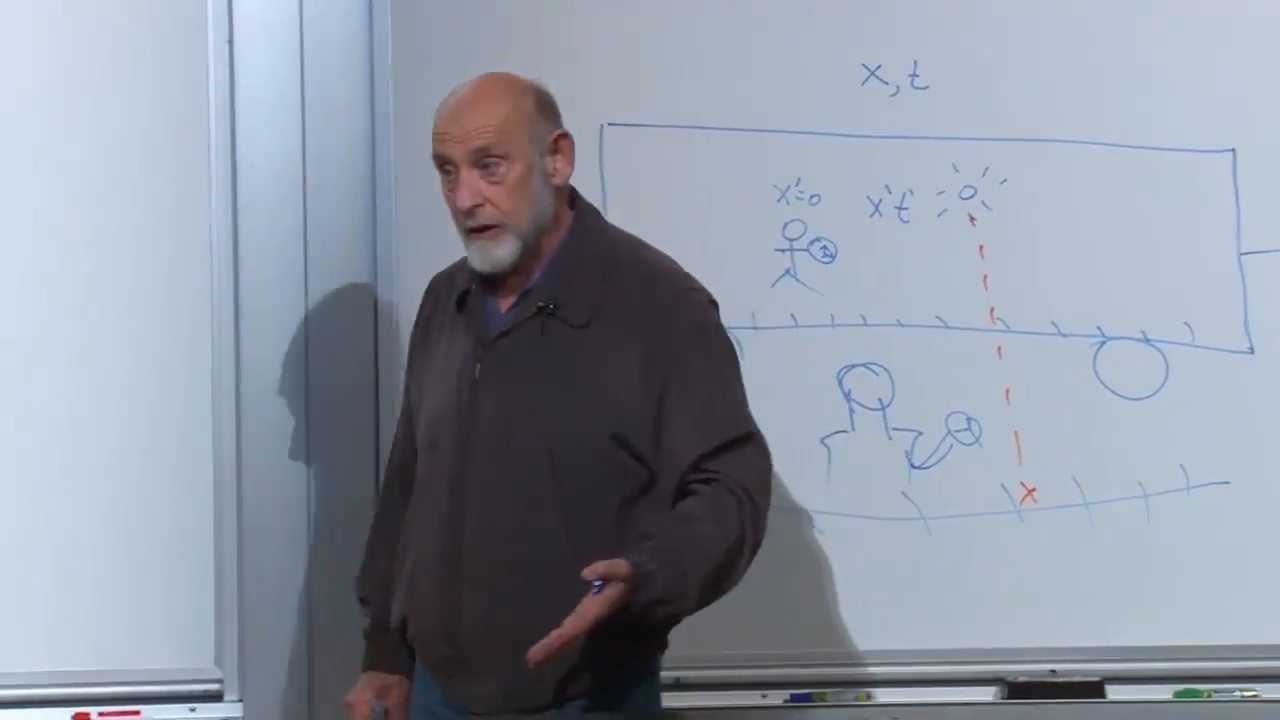
\includegraphics[width=0.90\textwidth]{lecture_02_figure_02.png}
\caption{역변환에도 같은 로렌츠 인자가 나타나며, 상대 속도의 부호만 반대다.}
\lectureframe{00:09:15}
\end{figure}

\(x\)축을 따른 부스트에서는 횡좌표가 변하지 않는다:
\begin{equation}
y'=y,
\qquad
z'=z.
\end{equation}

분모를 살펴보지 않아도 공간 방정식에서 상대 속도를 읽을 수 있다. 열차의 원점은 \(x'=0\)로 정의되므로,
\begin{equation}
x'=0
\quad\Longleftrightarrow\quad
x-vt=0
\quad\Longleftrightarrow\quad
x=vt.
\label{eq:sr2-origin-worldline}
\end{equation}
이 세계선에서 \(t\)의 계수가 역 좌표계로 나타낸 열차의 속도다.

\section{세 기준계와 부스트의 합성}

열차 안에 작은 장난감 자동차를 놓자. 열차는 역에 대해 속력 \(v\)로 움직이고, 자동차는 열차 승객에 대해 통로를 따라 속력 \(u\)로 움직인다. 자동차의 역에 대한 속력을 \(w\)라고 하자. 뉴턴 역학의 직관은 \(w=u+v\)라고 예상하지만, 답은 로렌츠 변환으로 구해야 한다.

이제 좌표계가 세 개다:
\begin{equation}
(x,t),\qquad (x',t'),\qquad (x'',t'').
\end{equation}
첫 번째는 역, 두 번째는 열차, 세 번째는 자동차에 속한다. 열차와 자동차 사이의 변환은 다음과 같다:
\begin{align}
x''&=\gamma_u(x'-ut'),&
t''&=\gamma_u(t'-ux'),
\label{eq:sr2-second-boost}\\
\gamma_u&=\frac{1}{\sqrt{1-u^2}}.
\end{align}

\begin{figure}[htbp]
\centering
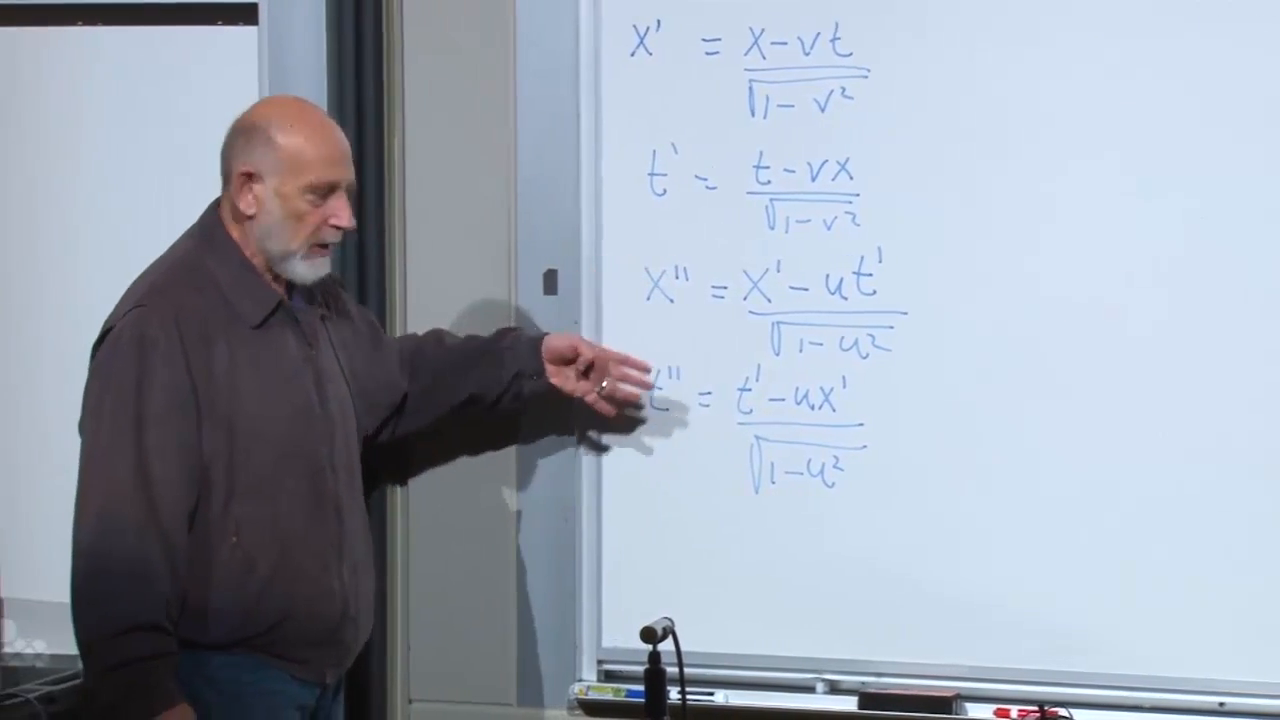
\includegraphics[width=0.90\textwidth]{lecture_02_figure_03.png}
\caption{역에서 프라임 좌표계로 가는 정변환에 이어, 프라임 좌표계에서 이중 프라임 좌표계로 가는 두 번째 로렌츠 변환을 적용한다.}
\lectureframe{00:14:55}
\end{figure}

\subsection{한 부스트를 다른 부스트에 대입하기}

\(w\)를 구하는 데에는 공간 방정식이면 충분하다. \eqref{eq:sr2-direct}를 \eqref{eq:sr2-second-boost}의 첫 번째 방정식에 대입하자:
\begin{align}
x''
&=\gamma_u(x'-ut')\\
&=\gamma_u\gamma_v\left[(x-vt)-u(t-vx)\right]\\
&=\gamma_u\gamma_v\left[(1+uv)x-(u+v)t\right].
\label{eq:sr2-composed-space}
\end{align}
\(uvx\) 항에 있는 두 음수 부호 때문에 그 항은 양수가 된다. 두 시간 항은 \(-(u+v)t\)로 합쳐진다.

\begin{figure}[htbp]
\centering
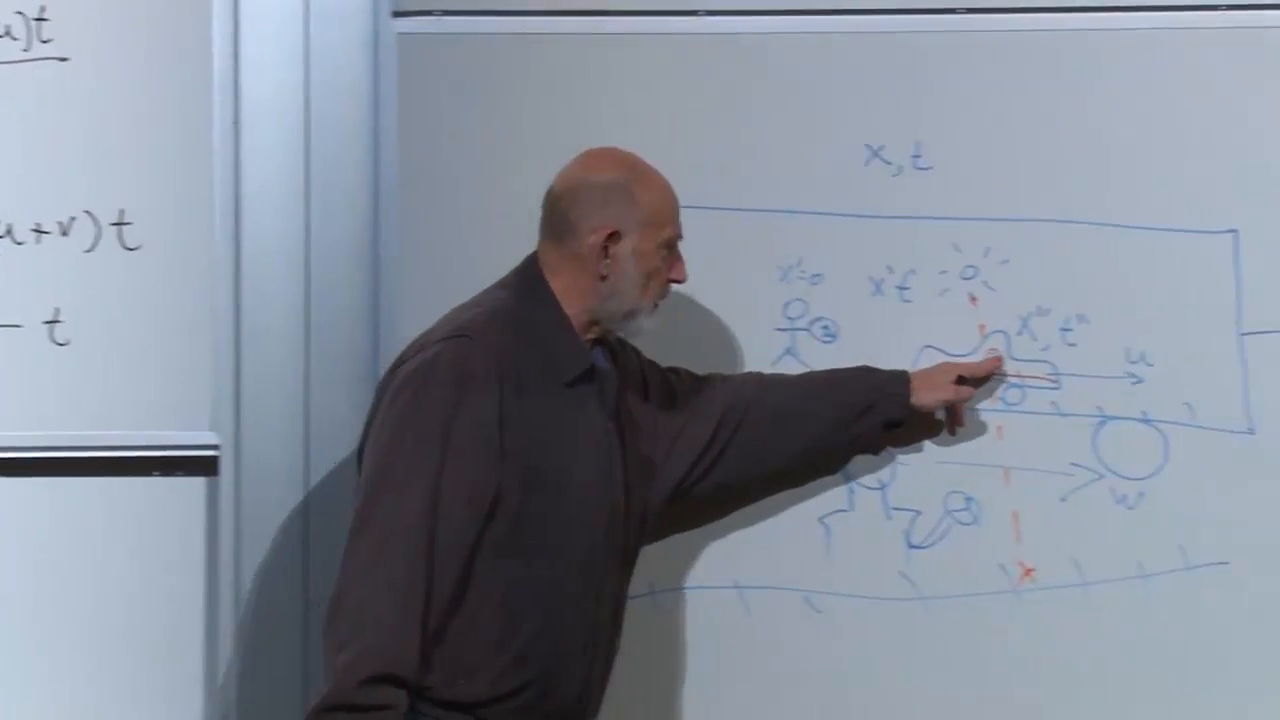
\includegraphics[width=0.91\textwidth]{lecture_02_figure_04.png}
\caption{합성된 부스트에서 \(x\) 항과 \(t\) 항을 모으기 전의 중첩 대입.}
\lectureframe{00:16:30}
\end{figure}

앞서와 마찬가지로, 움직이는 원점의 위치를 찾을 때 분모는 중요하지 않다. 꼬마 자동차는 \(x''=0\)에서 정지해 있으므로, \eqref{eq:sr2-composed-space}의 대괄호 안의 값은 영이어야 한다:
\begin{equation}
(1+uv)x-(u+v)t=0.
\end{equation}
따라서 정거장 좌표계에서 이 자동차의 세계선은
\begin{equation}
x=\frac{u+v}{1+uv}\,t,
\end{equation}
속도는
\begin{equation}
\boxed{w=\frac{u+v}{1+uv}}.
\label{eq:sr2-velocity-add-c1}
\end{equation}

\begin{figure}[htbp]
\centering
\includegraphics[width=0.91\textwidth]{lecture_02_figure_05.png}
\caption{정리한 분자와 세계선 \(x=[(u+v)/(1+uv)]t\)에서 합성된 속도를 알 수 있다.}
\lectureframe{00:19:30}
\end{figure}

시간 방정식도 일관되게 합성된다. 역에서 자동차로 가는 전체 변환은 로렌츠 변환의 형태를 갖는다:
\begin{align}
x''&=\gamma_w(x-wt),&
t''&=\gamma_w(t-wx),
\end{align}
여기서
\begin{equation}
\gamma_w=\frac{1}{\sqrt{1-w^2}}.
\end{equation}
실제로,
\begin{equation}
\gamma_w=\gamma_u\gamma_v(1+uv),
\end{equation}
이는 \eqref{eq:sr2-velocity-add-c1}를 대입하고 식을 정리하면 얻어진다. 따라서 같은 직선상에서 일어나는 두 부스트의 합성은 또 다른 같은 직선상의 부스트다.

\subsection{차원을 복원하기}

\begin{classroomqa}
\audiencequestion{보통 단위에서 분모 \(1+uv\)가 차원상 맞지 않는 이유는 무엇인가?}
\lecturerresponse{이는 \(c=1\)이어서 모든 속도가 빛의 속력에 대한 무차원 비율이 되기 때문에만 맞는 표현이다. 통상적인 단위에서는 곱이 \(uv/c^2\)로 나타나야 하며, 이 양은 무차원이다. \lecturetimestamp{00:21:11}}
\end{classroomqa}

차원을 고려한 속도 합성 법칙은 다음과 같다:
\begin{equation}
\boxed{
w=\frac{u+v}{1+\dfrac{uv}{c^2}}
}.
\label{eq:sr2-velocity-add}
\end{equation}

\begin{figure}[htbp]
\centering
\includegraphics[width=0.90\textwidth]{lecture_02_figure_06.png}
\caption{차원 일관성을 맞추면 곱 \(uv\) 아래에 \(c^2\)이 복원된다.}
\lectureframe{00:22:06}
\end{figure}

\(\lvert u\rvert,\lvert v\rvert\ll c\)일 때,
\begin{equation}
\frac{uv}{c^2}\ll 1,
\end{equation}
따라서
\begin{equation}
w\approx u+v.
\end{equation}
뉴턴식 덧셈은 별개의 법칙이 아니라 저속 근사다.

\subsection{두 가지 수치 영역}

먼저 다음 경우를 보자:
\begin{equation}
u=v=0.01c.
\end{equation}
단위 \(c=1\)에서,
\begin{equation}
w=\frac{0.02}{1.0001}\approx 0.019998.
\end{equation}
빛의 속력의 1퍼센트는 이미 약 \(3\times10^6\ {\rm m/s}\)이지만, 상대론적 보정은 만분의 일에 불과하다. 결과는 뉴턴 역학에서 예상하는 \(0.02c\)보다 약간 작다.

\begin{figure}[htbp]
\centering
\includegraphics[width=0.90\textwidth]{lecture_02_figure_07.png}
\caption{\(u=v=0.01c\)에서 분모는 1과 겨우 \(10^{-4}\)만큼 차이 난다.}
\lectureframe{00:24:23}
\end{figure}

이제 다음 경우를 보자:
\begin{equation}
u=v=0.9c.
\end{equation}
뉴턴 역학에서는 \(1.8c\)를 예측한다. 상대론에서는
\begin{equation}
\frac{w}{c}
=\frac{0.9+0.9}{1+0.9^2}
=\frac{1.8}{1.81}
\approx 0.9945.
\label{eq:sr2-fast-example}
\end{equation}

\begin{figure}[htbp]
\centering
\includegraphics[width=0.90\textwidth]{lecture_02_figure_08.png}
\caption{속력 \(0.9c\)인 두 물체의 속도를 합성하면 \(1.8/1.81\)가 되며, 여전히 빛의 속력보다 작다.}
\lectureframe{00:25:48}
\end{figure}

빛보다 느린 부스트를 연속해서 적용해도 \(c\)를 넘을 수 없다. \(u<c\)이고 \(v<c\)이면,
\begin{equation}
1-\frac{w}{c}
=
\frac{\left(1-\frac{u}{c}\right)
      \left(1-\frac{v}{c}\right)}
     {1+\frac{uv}{c^2}}
>0.
\end{equation}
부스트를 하나씩 더할 때마다 결과는 \(c\)에 더 가까워질 수 있지만, 결코 그 값을 넘지는 않는다. 극한값 \(u=c\)에서는,
\begin{equation}
w=\frac{c+v}{1+v/c}=c.
\end{equation}
빛의 속력은 합성 법칙의 고정점이다.

\section{좌표 측정은 시각적 모습과 다르다}

\begin{classroomqa}
\audiencequestion{열차에 유리 벽이 있다면, 역의 관측자는 승객과 장난감 자동차를 함께 바라보고 그 운동을 직접 알아낼 수 있는가?}
\lecturerresponse{로렌츠 변환은 공간 곳곳에 놓인 막대와 동기화된 시계를 사용해 얻는 좌표 측정에 관한 것이다. 시각적 영상에는 서로 다른 사건에서 관측자에게 도달하는 빛의 이동 시간이 서로 다르다는 점도 반영된다. 유리는 보이는 모습만 바꿀 뿐 좌표 관계는 바꾸지 않는다. 영상 하나를 동시각의 자료로 취급하면 상대론이 바로잡은 동시성 가정을 다시 들여오게 된다. \lecturetimestamp{00:27:53}}
\end{classroomqa}

그 순간에 누군가 사건을 보는지와 관계없이, 각 기준계에서 사건의 위치와 시간은 정해져 있다. 광학적 모습도 정당한 연구 대상이지만, 그러려면 각 사건에서 눈까지 빛이 이동하는 경로를 추적하는 별도의 계산이 필요하다. 변환 법칙 자체는 보편적이며 열차의 벽과 무관하다.

\section{세 공간 차원에서의 고유 간격}

두 사건으로 돌아가자. 첫 번째 사건은 원점에 있고, 두 번째 사건은 \((x,t)\)에 있다고 하자. 공간 차원이 하나일 때는,
\begin{equation}
\tau^2=t^2-x^2
\label{eq:sr2-interval-1d}
\end{equation}
단위 \(c=1\)에서 모든 관성계가 다음 값에 동의한다:
\begin{equation}
\tau^2
=t^2-x^2
=t'^2-x'^2
=t''^2-x''^2.
\end{equation}
좌표는 변하지만 고유 간격은 변하지 않는다.

시간꼴 분리에서는 시계가 두 사건 사이를 이동할 수 있다. 첫 사건에서 정오를 가리키던 시계가 두 번째 사건에서 가리키는 시각까지의 경과 시간은 고유시간 \(\tau\)이다. 어느 좌표계에서 간격을 계산하든 이 진술은 달라지지 않는다.

\begin{figure}[htbp]
\centering
\includegraphics[width=0.90\textwidth]{lecture_02_figure_09.png}
\caption{고유시간의 불변 관계 \(\tau^2=t^2-x^2\)를 상기한 뒤 횡방향을 다시 도입한다.}
\lectureframe{00:30:18}
\end{figure}

\subsection{공간 회전으로 횡방향 복원하기}

부스트를 다시 살펴보기 전에 공간축을 보통 방식으로 회전해 보자. \(x\)축 위에 놓이지 않은 점의 제곱 공간 거리는
\begin{equation}
r^2=x^2+y^2+z^2,
\end{equation}
이며, 보통의 피타고라스 정리에 따라 회전해도 변하지 않는다. 따라서 \(3+1\) 시공간 간격은
\begin{equation}
\boxed{
\tau^2=t^2-x^2-y^2-z^2
}.
\label{eq:sr2-interval-3d}
\end{equation}
\(c\)를 복원하면,
\begin{equation}
c^2\tau^2
=c^2t^2-x^2-y^2-z^2.
\end{equation}

\begin{figure}[htbp]
\centering
\includegraphics[width=0.90\textwidth]{lecture_02_figure_10.png}
\caption{피타고라스 정리에 따른 공간 거리를 이용하면 불변량이 \(t^2-x^2\)에서 \(t^2-x^2-y^2-z^2\)로 확장된다.}
\lectureframe{00:34:23}
\end{figure}

공간 회전과 로렌츠 부스트를 어떻게 조합하든 \eqref{eq:sr2-interval-3d}는 보존된다. 보통의 좌표축들은 성분은 서로 다르게 나타내지만 유클리드 거리는 같게 나타낸다. 관성 시공간 기준계들은 공간과 시간 성분은 서로 다르게 나타내지만 이 제곱들의 차는 같게 나타낸다. 이 불변량이 특수상대성이론의 핵심 기하학적 사실이다.

\begin{classroomqa}
\audiencequestion{승객이 장난감 자동차 대신 앞쪽으로 손전등을 비추면 열차 관측자와 역 관측자는 같은 빛의 속력을 얻는가?}
\lecturerresponse{\(u=c\)를 \eqref{eq:sr2-velocity-add}에 대입하자. 그러면 \(w=(c+v)/(1+v/c)=c\)이다. 단위 \(c=1\)에서는 그 비가 단순히 \((1+v)/(1+v)=1\)이다. 요구되는 대로 두 기준계 모두 정확히 같은 속력을 측정한다. \lecturetimestamp{00:35:53}}
\end{classroomqa}

따라서 앞서 제기된 유리 벽의 문제는 빛의 속력이 불변이라는 사실이 실패하는 경우가 아니다. 좌표 측정과 지연되어 보이는 시각적 영상, 궁극적으로는 동시성에 관한 혼동이다.

\section{빛살과 빛원뿔}

한 공간 차원에서 오른쪽과 왼쪽으로 진행하는 빛살은 다음을 만족한다:
\begin{equation}
x=\pm t.
\end{equation}
이 빛살의 시공간 간격은 영이다:
\begin{equation}
t^2-x^2=0.
\end{equation}
유클리드 거리와 달리, 시공간 간격이 영이라고 해서 두 사건이 일치해야 하는 것은 아니다. 이는 빛 신호가 두 사건을 연결할 수 있음을 뜻한다.

공간 방향을 모두 복원하면 빛살은 다음을 만족한다:
\begin{equation}
t^2-x^2-y^2-z^2=0,
\label{eq:sr2-null}
\end{equation}
또는
\begin{equation}
r=t
\end{equation}
단위 \(c=1\)에서 미래 방향으로 진행하는 빛에 대해 성립한다.

\begin{figure}[htbp]
\centering
\includegraphics[width=0.90\textwidth]{lecture_02_figure_11.png}
\caption{어느 공간 방향으로 진행하든 빛은 \(t^2-(x^2+y^2+z^2)=0\)을 만족하는 영 궤적을 따른다.}
\lectureframe{00:39:28}
\end{figure}

\(1+1\)차원에서는 영집합이 \(45^\circ\)인 두 직선이다. 공간 차원 둘과 시간 차원 하나에서는 원뿔이 된다. 공간 차원이 셋이면 칠판에 온전히 그릴 수 없지만, 이를 정의하는 방정식은 그대로다.

미래 빛원뿔은 원점에서 방출된 빛이 도달할 수 있는 사건들로 이루어진다. 과거 빛원뿔은 빛이 원점에 도달할 수 있는 사건들로 이루어진다. 하나는 다른 하나를 시간에 대해 뒤집은 것이다.

\begin{figure}[htbp]
\centering
\includegraphics[width=0.90\textwidth]{lecture_02_figure_12.png}
\caption{\(45^\circ\)인 영광선들이 더 높은 차원의 시공간 그림에서 미래와 과거 빛원뿔을 이룬다.}
\lectureframe{00:40:47}
\end{figure}

\begin{classroomqa}
\audiencequestion{뉴턴 역학의 갈릴레이 변환에서 이에 대응하는 불변량은 무엇인가?}
\lecturerresponse{시간 간격 자체다. 뉴턴 역학의 관측자들은 공간 변위에는 동의하지 않지만 모두 \(\Delta t\)에는 동의한다. 상대론은 보편적 시간을 포기하고 그 자리에 불변 시공간 간격을 둔다. \lecturetimestamp{00:41:53}}
\end{classroomqa}

\section{공간 벡터에서 사차원 벡터로}

여기서 벡터는 양자 상태 벡터가 아니라 기하학적 벡터다. 보통 공간에서 두 점 사이의 변위에는 크기와 방향이 있다. 벡터의 꼬리를 옮겨 원점에 놓아도 벡터는 바뀌지 않으며, 그 세 성분은 다음과 같이 쓸 수 있다:
\begin{equation}
x^i=(x^1,x^2,x^3)=(x,y,z),
\qquad i=1,2,3.
\end{equation}
라틴 지표 \(i\)는 공간 방향만을 나타낸다.

사건에는 시간이라는 성분이 하나 더 필요하다. 따라서 시공간 위치는 다음과 같이 쓴다:
\begin{equation}
x^\mu=(x^0,x^1,x^2,x^3)=(t,x,y,z),
\qquad \mu=0,1,2,3.
\label{eq:sr2-four-position}
\end{equation}
역사적 관례에 따라 시간은 네 번째 성분이 아니라 영 번째 성분으로 둔다:
\begin{equation}
x^0=t,\qquad x^1=x,\qquad x^2=y,\qquad x^3=z.
\end{equation}
\(\mu\)와 같은 그리스 첨자는 시공간 성분을, \(i\)와 같은 라틴 첨자는 공간 성분을 나타낸다.

\begin{figure}[htbp]
\centering
\includegraphics[width=0.90\textwidth]{lecture_02_figure_13.png}
\caption{공간 성분 \(x^i\)를 네 성분으로 이루어진 시공간 위치 \(x^\mu=(x^0,x^1,x^2,x^3)\)로 확장한다.}
\lectureframe{00:46:05}
\end{figure}

불변량은 다음과 같이 된다:
\begin{equation}
\tau^2
=(x^0)^2-(x^1)^2-(x^2)^2-(x^3)^2.
\end{equation}
이 표기법 자체가 새로운 물리를 더하는 것은 아니다. 그 장점은 로렌츠 변환이 공간 벡터에 회전이 작용하듯 네 성분 모두에 선형으로 작용한다는 데 있다.

\begin{classroomqa}
\audiencequestion{변환이 선형이므로 열벡터에 작용하는 행렬로 나타낼 수 있는가?}
\lecturerresponse{그렇다. \(x\)축 방향 부스트에서는 \(\gamma_v\begin{pmatrix}1&-v\\-v&1\end{pmatrix}\)가 \((t,x)^{\mathsf T}\)에 작용하고, \(y\)와 \(z\)는 변하지 않는다. 로렌츠 변환을 합성하고 정리하는 데 행렬 표기가 자연스럽다. \lecturetimestamp{00:48:14}}
\end{classroomqa}

구체적으로 쓰면,
\begin{equation}
\begin{pmatrix}
t'\\x'\\y'\\z'
\end{pmatrix}
=
\begin{pmatrix}
\gamma_v&-\gamma_v v&0&0\\
-\gamma_v v&\gamma_v&0&0\\
0&0&1&0\\
0&0&0&1
\end{pmatrix}
\begin{pmatrix}
t\\x\\y\\z
\end{pmatrix}.
\label{eq:sr2-boost-matrix}
\end{equation}

\section{변위와 사차원 속도}

한 사건의 위치에서 입자 세계선의 짧은 구간으로 옮겨가 보자. 사차원 변위는 다음과 같다:
\begin{equation}
\Delta x^\mu
=(\Delta t,\Delta x,\Delta y,\Delta z).
\end{equation}
변위가 작다고 할 때 미적분학의 관점으로 다가가며, \(\Delta x^\mu\)는 \(dx^\mu\)가 된다. 지금은 기하를 명확히 보여 주는 유한한 변위 표기를 사용한다.

시간꼴 세계선을 따라 고유시간 증분은 다음을 만족한다:
\begin{equation}
(\Delta\tau)^2
=(\Delta t)^2-(\Delta x)^2-(\Delta y)^2-(\Delta z)^2.
\label{eq:sr2-proper-increment}
\end{equation}
보통의 속도는 공간 변위를 좌표 시간으로 나누며 세 성분을 갖는다. 사차원 속도는 대신 사차원 변위를 불변 고유시간으로 나눈다:
\begin{equation}
u^\mu
=\frac{\Delta x^\mu}{\Delta\tau}
\quad\longrightarrow\quad
\boxed{
u^\mu=\frac{dx^\mu}{d\tau}
}.
\label{eq:sr2-four-velocity}
\end{equation}

\begin{figure}[htbp]
\centering
\includegraphics[width=0.90\textwidth]{lecture_02_figure_14.png}
\caption{세계선의 한 구간은 \(\Delta x^\mu\), 그 불변량 \(\Delta\tau\), 그리고 사차원 속도 \(u^\mu=\Delta x^\mu/\Delta\tau\)를 정의한다.}
\lectureframe{00:52:42}
\end{figure}

이 양은 네 성분을 가지며 사차원 벡터처럼 변환된다. 이것과 보통의 삼차원 속도가 어떻게 관계되는지는 다음 질문이며, 여기서는 일부러 답을 미뤄 둔다. 이 관계를 밝히면 상대론적 운동량, 에너지, 가속도, 그리고 마침내 \(F=ma\)의 상대론적 일반화로 나아가게 된다.